\chapter{Adresses MAC et probes requests}
\label{ch:probe_req}

Afin de pouvoir détecter et tracer les différents périphériques réseau présents
pendant les scans, il est impératif de pouvoir les identifier de manière unique et irrévocable.

Pour cela, nous allons utiliser l'adresse MAC. 
Cet identifiant unique peut être récupéré de plusieurs manières, mais ce sont les \textbf{probe requests}
qui vont nous offrir la plus grande souplesse. 

Explorons ces deux concepts.

\section{Adresse MAC, un identifiant pas si unique}

\subsection{Définition:}~\cite{wiki:mac}

"Une adresse MAC (Media Access Control1), parfois nommée adresse physique, est un identifiant physique 
stocké dans une carte réseau ou une interface réseau similaire. À moins qu'elle n'ait été modifiée par l'utilisateur, elle est unique au monde. 

MAC constitue la partie inférieure de la couche de liaison (couche 2 du modèle OSI). Elle insère et traite ces adresses au sein des trames transmises. Elle est parfois appelée adresse ethernet, 
UAA (Universally Administered Address), BIA (Burned-In Address), MAC-48 ou EUI-48."

\subsection{Format}

Les 48 bits d'une adresse sont schématisés sur la figure ~\ref{fig:macstruct} et formatés comme suit :

\begin{figure}[H]
	\centering
	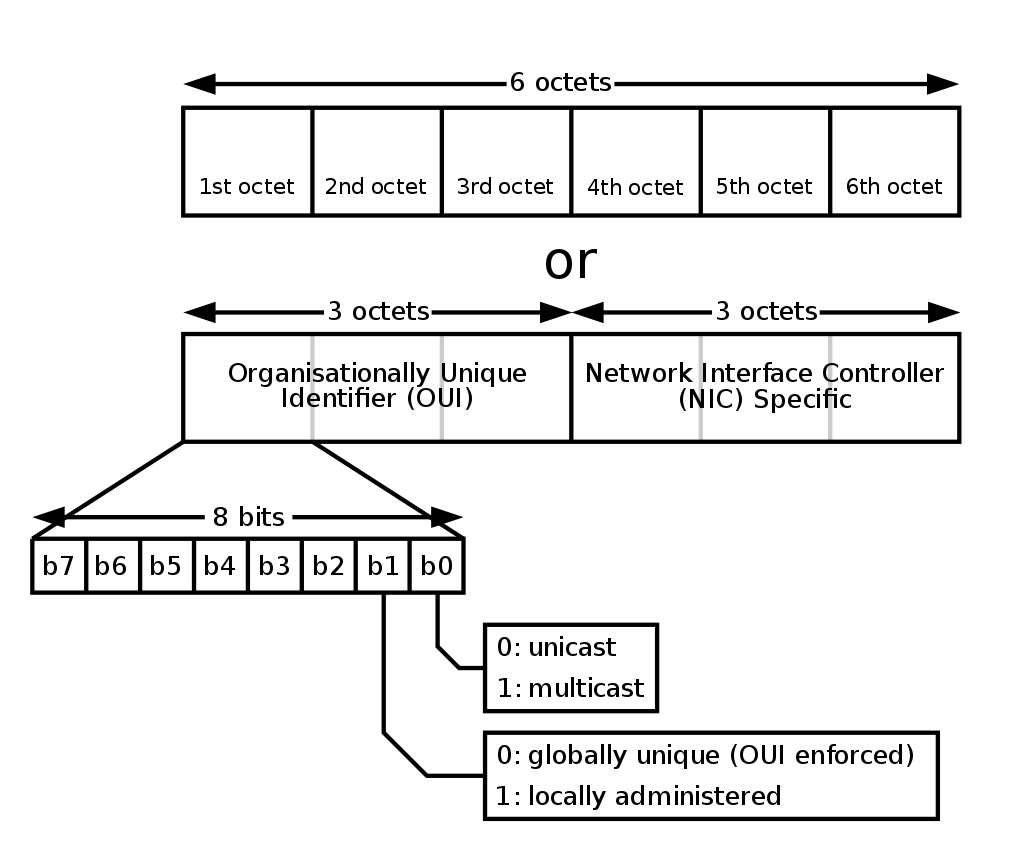
\includegraphics[width=12cm]{images/probe/mac_struc.png}
	\caption{Structure de l'adresse MAC}
	\label{fig:macstruct}
\end{figure}

Les 3 octets de poids faible sont variables et change pour chaque carte mère, c'est ce qui rend chaque adresse du même
constructeur unique, il s'agit du \textbf{NIC}.

Les 3 octets de poids fort sont presque fixes pour chaque constructeur, il s'agit du \textbf{OUI}.
Toutefois, les deux bits de poids faible du premier octet peuvent varier (b1 et b0 sur l'illustration).

b0 indique si l'adresse est individuelle, auquel cas le bit sera à 0 (pour une machine unique, unicast) 
ou de groupe (multicast ou broadcast), en passant le bit à 1.

b1 indique 0 si l'adresse est universelle (conforme au format de l'IEEE) ou 
locale, 1 pour une adresse administrée localement (ce bit sera crucial concernant l'analyse de la randomisation)

\subsection{Problèmes de vie privée et randomisation}
La propriété d'unicité des adresses MAC soulève évidemment des problématiques liées à la vie privée. 
Par exemple, selon les dires d'Edward Snowden, la NSA se servait des adresses MAC afin de
monitorer les déplacements d'individus.~\cite{hackernews:snowdan}

Le sujet de ce travail de bachelor soulève les même problématiques. Par conséquent, certaines marques
ont mis en place la \textbf{MAC Address randomization}.

\subsection{Randomisation des adresses MAC}~\cite{connected:macrandom}

Depuis 2014, de plus en plus de constructeurs ont adoptés des mesures
afin de protéger la véritable adresse MAC de l'appareil. 

\begin{itemize}
    \item iOS à partir d’iOS 8 ;
    \item Windows depuis Windows 10 ;
    \item Android depuis Android 6.0 (un patch gère également Android 5.0 pour certains appareils) ;
    \item certains drivers Linux depuis le kernel 3.18.
\end{itemize}

L'objectif étant de varier suffisamment régulièrement l'adresse pour empêcher le traçage. 
Le processus de randomisation n'étant pas strictement standardisé, l'implémentation peut varier pour chaque constructeur. 

Certaines de ces implémentations sont bonnes (iOS randomise les 6 octets de l'adresse MAC, sauf b1 et b0) alors que d'autres le sont moins (Android possède des OUI fixes pendant la randomisation, ce qui 
permet déjà la divulgation d'informations sur l'appareil.)

\subsubsection{Problèmes liés à l'implémentation de la randomisation}

Bien que le concept de randomisation soit une bonne avancée dans le domaine de la privacy, quelques
problèmes d'implémentation ont mitigé cette dernière. 

Parmi les problèmes récurrents, il a été trouvé:
\begin{itemize}
	\item Mauvais PRNG (le biais permet de faire des liens logiques entre les adresses)
	\item Numéros de séquence augmentant de manière monotone, permettant de faire le lien entre deux adresses aléatoires (cf~\ref{fig:seqnumber})
	\item Les adresses réelles sont parfois divulguées (e.g si l'écran est allumé)
	\item Les timings de scans des appareils peuvent permettre un rapprochement entre plusieurs adresses
	\item Fingerprinting possible à l'aide des Informations Elements (IE)
	\item Beaucoup de méthodes de randomisation ne sont utilisées que lors du scan. Lorsque l'appareil est connecté, ce dernier utilise à nouveau
	sa vraie adresse physique.
\end{itemize} 

Tous ces points s'améliorent avec le temps. 
Par exemple, la nouvelle version d'iOS (14) datant de l'été 2020 permet la randomisation même lorsque l'appareil est connecté.
Cette feature est d'ailleurs mise en avant par Apple, au travers des notifications. \cite{APPLESUPPPRIVATE} 

\begin{figure}[H]
	\centering
	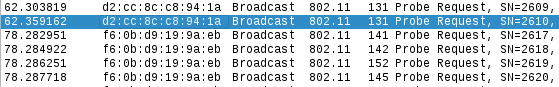
\includegraphics[width=12cm]{images/probe/sn.png}
	\caption{Le changement d'adresse MAC aux lignes 2 et 3 peut être déduit à cause du séquence number proche.}
	\source{~\cite{connected:macrandom}}
	\label{fig:seqnumber}
\end{figure}

\subsection{Détection passive de la randomisation}

\subsubsection{Le bit Locally Assigned}
Le travail WiFace utilise plusieurs méthodes pour détecter la randomisation des adresses MAC. 
La première consiste simplement à contrôler le bit \textbf{b1}, si ce dernier est à 1, cela implique qu'il
y a de grandes chances que l'adresse soit aléatoire. Cependant, ce n'est pas totalement vrai, c'est pourquoi
d'autres techniques sont employées en concert avec celle-ci. 

Dans un corpus datant de fin 2015, l'étude ~\cite{ASMARMD} a demontré les statistiques visibles dans le tableau~\ref{tab:locally_stats}: 

\begin{table}[H]
	\resizebox{\textwidth}{!}{%
	\begin{tabular}{@{}lll@{}}
	\toprule
	\textbf{Category} & \textbf{Subcategory} & \textbf{Number of MACs} \\ \midrule
	\multirow{5}{*}{Locally Assigned} & Total & 1400753 \\
	 & Randomized & 1388656 \\
	 & Service & 4371 \\
	 & Malformed & 6895 \\
	 & Unknown & 831 \\ \bottomrule
	\end{tabular}%
	}
	\caption{Statistiques sur la randomisation - Locally Assigned bit}
	\label{tab:locally_stats}
	\end{table}

Près de 99\% des adresses assignées localement étaient également aléatoires. La consultation
du bit b1 est donc une bonne estimation heuristique. Il est tout de fois intéressant de pouvoir afiner
la détection afin d'obtenir d'autres informations sur le périphérique. 

\subsubsection{Le préfixe DA:A1:19}
Ce préfixe peut être retrouvé lors de la randomisation des adresses MAC sous Android.
Il s'agit d'un CID hardcodé dans un fichier de configuration de l'OS. Cette valeur sera donc utilisée "par défaut"
lors de la randomisation Android. Dans ce même corpus, 52685 adresses étaient concernées.

\subsubsection{Le préfixe 92:68:C3}
Ce CID a également été observé sur un petit sous-ensemble des appareils. Il est possédé par Motorola et venait remplacer
celui d'Android.

\section{Les probes requests}

Les adresses MAC, aléatoires ou non, sont transmises dans chaque trame MAC, ainsi que bien d'autres
informations. Voici leur structure:

\begin{figure}[H]
	\centering
	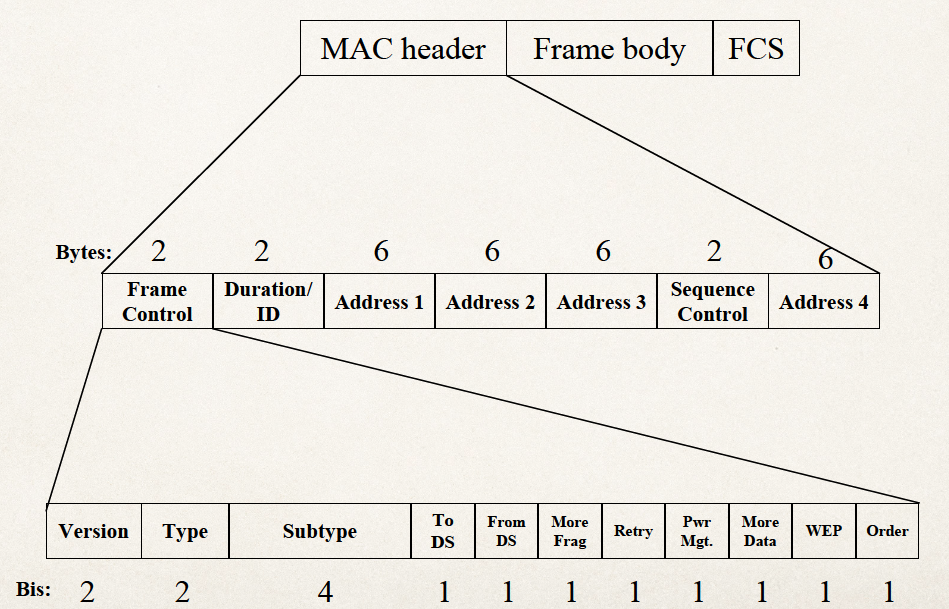
\includegraphics[width=14cm]{images/probe/mac_frame.png}
	\caption{Structure d'une trame MAC}
	\label{fig:macframe}
\end{figure}

On retrouve notamment les adresses MAC de source et de destination dans les champs Address[1|2|3].
Malheureusement, pour qu'un appareil diffuse des trames de \textbf{données}, il faut qu'il soit associé avec un point d'accès. 
Il existe cependant les trames de \textbf{management}. Le champ "Subtype" (cf figure \ref{fig:macframe}) définit justement
la nature de ces frames. 

Voici les trames de management principales:
\begin{itemize}
    \item Beacon
    \item Probe request \& response
    \item Authentification
    \item Association request \& response
    \item Re-association request \& response
    \item Disassociation
    \item De-Authentification
\end{itemize}

Les trames \textbf{Beacon} sont utilisées par les points d'accès pour signaler leur existence. 

Les trames d'\textbf{(De-)Authentification} sont utilisées par une station et un point d'accès afin d'établir leur identité (pas de chiffrement à ce stade).

Les trames d'\textbf{(Dis|Re)Association} sont utilisées pour lier un AP et une station après l'authentification.

Les trames de \textbf{Probing} servent à un client (request) à demander à un AP les informations nécessaires à la connexion (e.g le canal).
L'AP concerné envoie alors une probe response avec les informations. 

Une probe request peut être dirigée (un SSID spécifique est spécifié, on l'appelle alors "directed probe request") ou alors aucun SSID n'est spécifié, dans ce cas
on l'appelle "null probe request"

Pour notre solution de scanning, nous cherchons une trame qui n'a pas d'interaction direct avec un access point préexistant
et qui est envoyée par le client. Parmi les trames de management mentionnées, seules les probe requests respectent ces deux contraintes.

Un autre avantage des probe request est que ces dernières sont envoyées très régulièrement (plusieurs fois par minute)
afin de permettre à l'appareil de trouver rapidement les WiFi disponibles. Elles sont même envoyées en rafale ("burst") afin de couvrir
un maximum de canaux 802.11.

Une capture de probe request dirigée peut être observée sur la capture~\ref{fig:directedprobe} :
\begin{figure}[H]
	\centering
	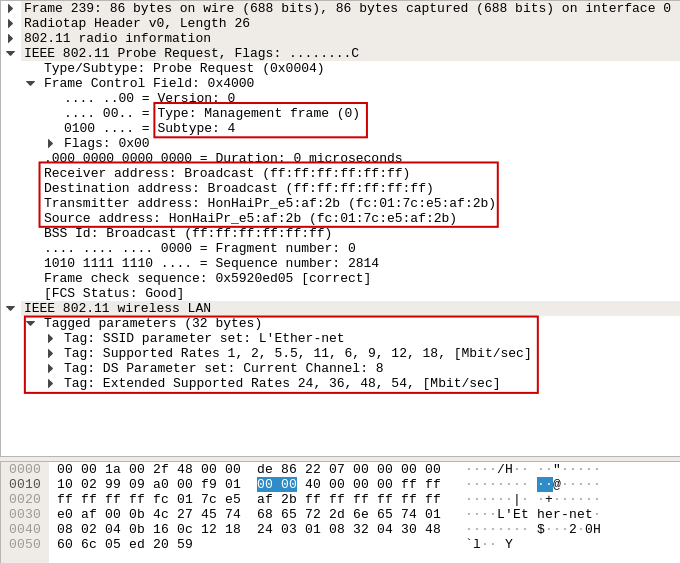
\includegraphics[width=14cm]{images/probe/directed_probe.png}
	\caption{Probe request dirigée}
	\label{fig:directedprobe}
\end{figure}

On y trouve le sous-type de la trame de management qui identifie les Probe requests (4), l'adresse de destination (broadcast)
, l'adresse source (un téléphone Honor 8) et différentes informations dont le \textbf{SSID} recherché : "L'Ether-net"

Les même informations sont disponibles pour une null probe request (figure~\ref{fig:nulldprobe}), mais le SSID est remplacé par un wildcard:
\begin{figure}[H]
	\centering
	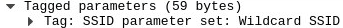
\includegraphics[width=14cm]{images/probe/null_probe_cropped.png}
	\caption{null-probe request}
	\label{fig:nulldprobe}
\end{figure}

Il est intéressant de noter que des informations peuvent parfois être déduites des probes requests dirigées.
La plupart du temps, les requêtes sont dirigées car l'appareil s'est déjà connecté au réseau concerné. 
Si le nom du réseau est connu et assez unique, il devient alors possible de déduire où l'appareil se situait par le passé.
Par exemple, sur la figure \ref{fig:directedprobe}, le SSID est l'ancien nom de mon réseau, je peux donc en déduire qu'il s'agit
d'un de mes appareils, et qu'il n'est pas récent. 

Cette technique est aussi utilisée afin de découvrir des réseaux cachés (il s'agit de réseaux qui ne répondent pas aux null probe requests et qui n'envoient pas de beacons).

